\documentclass[../SperimentazioniPratiche.tex]{subfiles}

\begin{document}

\section{Allestimento impianti}
\label{sec:AllestimentoImpianto}

	\subsection{Registro impianti}
	
	\begin{table} [h]
		\centering
		\begin{tabular}{lcc}
			\toprule
			\textbf{Identificativo} & \textbf{Edificio} & \textbf{Numero Piani}		\\
			\toprule
			\hyperref[subsec:Impianto1]{Impianto1} & Torre Archimede & 2 \\
			\bottomrule
		\end{tabular}
		\caption{Registro degli impianti}
		\label{tab:RegistroImpianti}
	\end{table}
	
	
	\newpage
	\subsection{Impianto1}
	\label{subsec:Impianto1}
		L'\textbf{Impianto1} identifica l'impostazione dei beacon nel piano terra e nel primo piano dell'edificio \textbf{Torre Archimede} situato in Via Trieste, 63 - 35121 Padova.
		
		\subsubsection{Configurazione beacon}
		Beacon utilizzati per l'allestimento dell'impianto di prova:
		\begin{itemize}
			\item[] \textbf{Kontakt.io Smart Beacon}.
		\end{itemize}
		Dati per la configurazione dei beacon facenti parte dell'impianto:
		\begin{itemize}
			\item[] \textbf{UUID:} 19235dd2-574a-4702-a42e-caccac06e325;
			\item[] \textbf{Major:} 666;
			\item[] \textbf{Advertaising interval:} 350 ms;
			\item[] \textbf{Potenza:} 0.
		\end{itemize}

		
		Di seguito sono elencate le schede di ogni beacon utilizzato per la costruzione dell'impianto. Ogni scheda è strutturata dai seguenti campi
		\begin{itemize}
			\item Il \textbf{titolo} di ogni scheda rappresenta il \textbf{Major} impostato a tale beacon;
			\item All'interno di ogni scheda:
			\begin{itemize}
				\item L'\textbf{Identificativo} rappresenta l'id del produttore assegnato al beacon per poterlo riconoscere;
				\item I \textbf{Point Of Interest} elencano tutti i POI che appartengono all'area coperta dal beacon (Region Of Interest).
			\end{itemize}
		\end{itemize}
		
		\newpage
		\paragraph{Piano terra}		
		
			\paragraph*{}
			\label{00000}
			\begin{tcolorbox}[fonttitle=\bfseries, 
								adjusted title={\Large Beacon 00000},
								sharp corners=south,
								colback=white, 
								colframe=white!50!blue!75!black]
								
				\begin{description}%[leftmargin=0.9cm,labelwidth=!]
					\item[Identificativo]: fO2c

					\tcbline					
					
					\item[Point Of Interest:] \ \par
					\begin{itemize}
						\item Entrata Torre A
					\end{itemize}					   				
				\end{description}  				
			\end{tcolorbox}
			
			\paragraph*{}
			\label{00001}
			\begin{tcolorbox}[fonttitle=\bfseries, 
								adjusted title={\Large Beacon 00001},
								sharp corners=south,
								colback=white, 
								colframe=white!50!blue!75!black]
								
				\begin{description}%[leftmargin=0.9cm,labelwidth=!]
					\item[Identificativo]: KTUd

					\tcbline					
					
					\item[Point Of Interest:] \ \par
					\begin{itemize}
						\item Entrata Torre B
					\end{itemize}					   				
				\end{description}  				
			\end{tcolorbox}
			
			\paragraph*{}
			\label{00002}
			\begin{tcolorbox}[fonttitle=\bfseries, 
								adjusted title={\Large Beacon 00002},
								sharp corners=south,
								colback=white, 
								colframe=white!50!blue!75!black]
								
				\begin{description}%[leftmargin=0.9cm,labelwidth=!]
					\item[Identificativo]: Ubuc

					\tcbline					
					
					\item[Point Of Interest:] \ \par
					\begin{itemize}
						\item Entrata Torre C
					\end{itemize}					   				
				\end{description}  				
			\end{tcolorbox}
			
			\paragraph*{}
			\label{00003}
			\begin{tcolorbox}[fonttitle=\bfseries, 
								adjusted title={\Large Beacon 00003},
								sharp corners=south,
								colback=white, 
								colframe=white!50!blue!75!black]
								
				\begin{description}%[leftmargin=0.9cm,labelwidth=!]
					\item[Identificativo]: pZtz

					\tcbline					
					
					\item[Point Of Interest:] \ \par
					\begin{itemize}
						\item Entrata Torre D
					\end{itemize}					   				
				\end{description}  				
			\end{tcolorbox}
			

		% -------------------- Cambio piano --------------------			
			
		\paragraph{Primo piano}			
			
			\paragraph*{}
			\label{01000}
			\begin{tcolorbox}[fonttitle=\bfseries, 
								adjusted title={\Large Beacon 01000},
								sharp corners=south,
								colback=white, 
								colframe=white!50!blue!75!black]
								
				\begin{description}
					\item[Identificativo]: Y4MM

					\tcbline					
					
					\item[Point Of Interest:] \ \par
					\begin{itemize}
						\item 1AD100
						\item Toilette donne AD 1
						\item 1A150
					\end{itemize}					   				
				\end{description}  				
			\end{tcolorbox}
			
			\paragraph*{}
			\label{01001}
			\begin{tcolorbox}[fonttitle=\bfseries, 
								adjusted title={\Large Beacon 01001},
								sharp corners=south,
								colback=white, 
								colframe=white!50!blue!75!black]
								
				\begin{description}
					\item[Identificativo]: nOGn

					\tcbline					
					
					\item[Point Of Interest:] \ \par
					\begin{itemize}
						\item 1BC50
						\item Toilette uomini BC 1
						\item 1A150
					\end{itemize}					   				
				\end{description}  				
			\end{tcolorbox}
			
			\paragraph*{}
			\label{01002}
			\begin{tcolorbox}[fonttitle=\bfseries, 
								adjusted title={\Large Beacon 01002},
								sharp corners=south,
								colback=white, 
								colframe=white!50!blue!75!black]
								
				\begin{description}
					\item[Identificativo]: ITg6

					\tcbline					
					
					\item[Point Of Interest:] \ \par
					\begin{itemize}
						\item 1BC45
						\item Toilette donne BC 1
						\item 1C150
					\end{itemize}					   				
				\end{description}  				
			\end{tcolorbox}
			
			\paragraph*{}
			\label{01003}
			\begin{tcolorbox}[fonttitle=\bfseries, 
								adjusted title={\Large Beacon 01003},
								sharp corners=south,
								colback=white, 
								colframe=white!50!blue!75!black]
								
				\begin{description}
					\item[Identificativo]: 4CUJ

					\tcbline					
					
					\item[Point Of Interest:] \ \par
					\begin{itemize}
						\item 1AD100
						\item Toilette uomini AD 1
						\item 1C150
					\end{itemize}					   				
				\end{description}  				
			\end{tcolorbox}
			
			\paragraph*{}
			\label{01004}
			\begin{tcolorbox}[fonttitle=\bfseries, 
								adjusted title={\Large Beacon 01004},
								sharp corners=south,
								colback=white, 
								colframe=white!50!blue!75!black]
								
				\begin{description}
					\item[Identificativo]: 7imi

					\tcbline					
					
					\item[Point Of Interest:] \ \par
					\begin{itemize}
						\item Nessuno
					\end{itemize}					   				
				\end{description}  				
			\end{tcolorbox}
			
			\paragraph*{}
			\label{01005}
			\begin{tcolorbox}[fonttitle=\bfseries, 
								adjusted title={\Large Beacon 01005},
								sharp corners=south,
								colback=white, 
								colframe=white!50!blue!75!black]
								
				\begin{description}
					\item[Identificativo]: wESv

					\tcbline					
					
					\item[Point Of Interest:] \ \par
					\begin{itemize}
						\item Nessuno
					\end{itemize}					   				
				\end{description}  				
			\end{tcolorbox}
			
			\paragraph*{}
			\label{01006}
			\begin{tcolorbox}[fonttitle=\bfseries, 
								adjusted title={\Large Beacon 01006},
								sharp corners=south,
								colback=white, 
								colframe=white!50!blue!75!black]
								
				\begin{description}
					\item[Identificativo]: Zmb4

					\tcbline					
					
					\item[Point Of Interest:] \ \par
					\begin{itemize}
						\item Nessuno
					\end{itemize}					   				
				\end{description}  				
			\end{tcolorbox}
			
			\paragraph*{}
			\label{01007}
			\begin{tcolorbox}[fonttitle=\bfseries, 
								adjusted title={\Large Beacon 01007},
								sharp corners=south,
								colback=white, 
								colframe=white!50!blue!75!black]
								
				\begin{description}
					\item[Identificativo]: GSbJ

					\tcbline					
					
					\item[Point Of Interest:] \ \par
					\begin{itemize}
						\item Nessuno
					\end{itemize}					   				
				\end{description}  				
			\end{tcolorbox}
			
		
		
		\newpage
		\subsubsection{Planimetrie e posizionamento}
			Ogni beacon è stato posizionato sul soffitto nel primo piano dell'edificio nei punti indicati dalla planimetria \ref{fig:PrimoPiano} mentre per il piano terra \ref{fig:PianoTerra} i beacon sono stati posizionanti sulla parete ad altezza 2,30 metri. Per attaccarli è stato utilizzato del normale nastro adesivo in carta.
			
			\begin{figure}[h]
				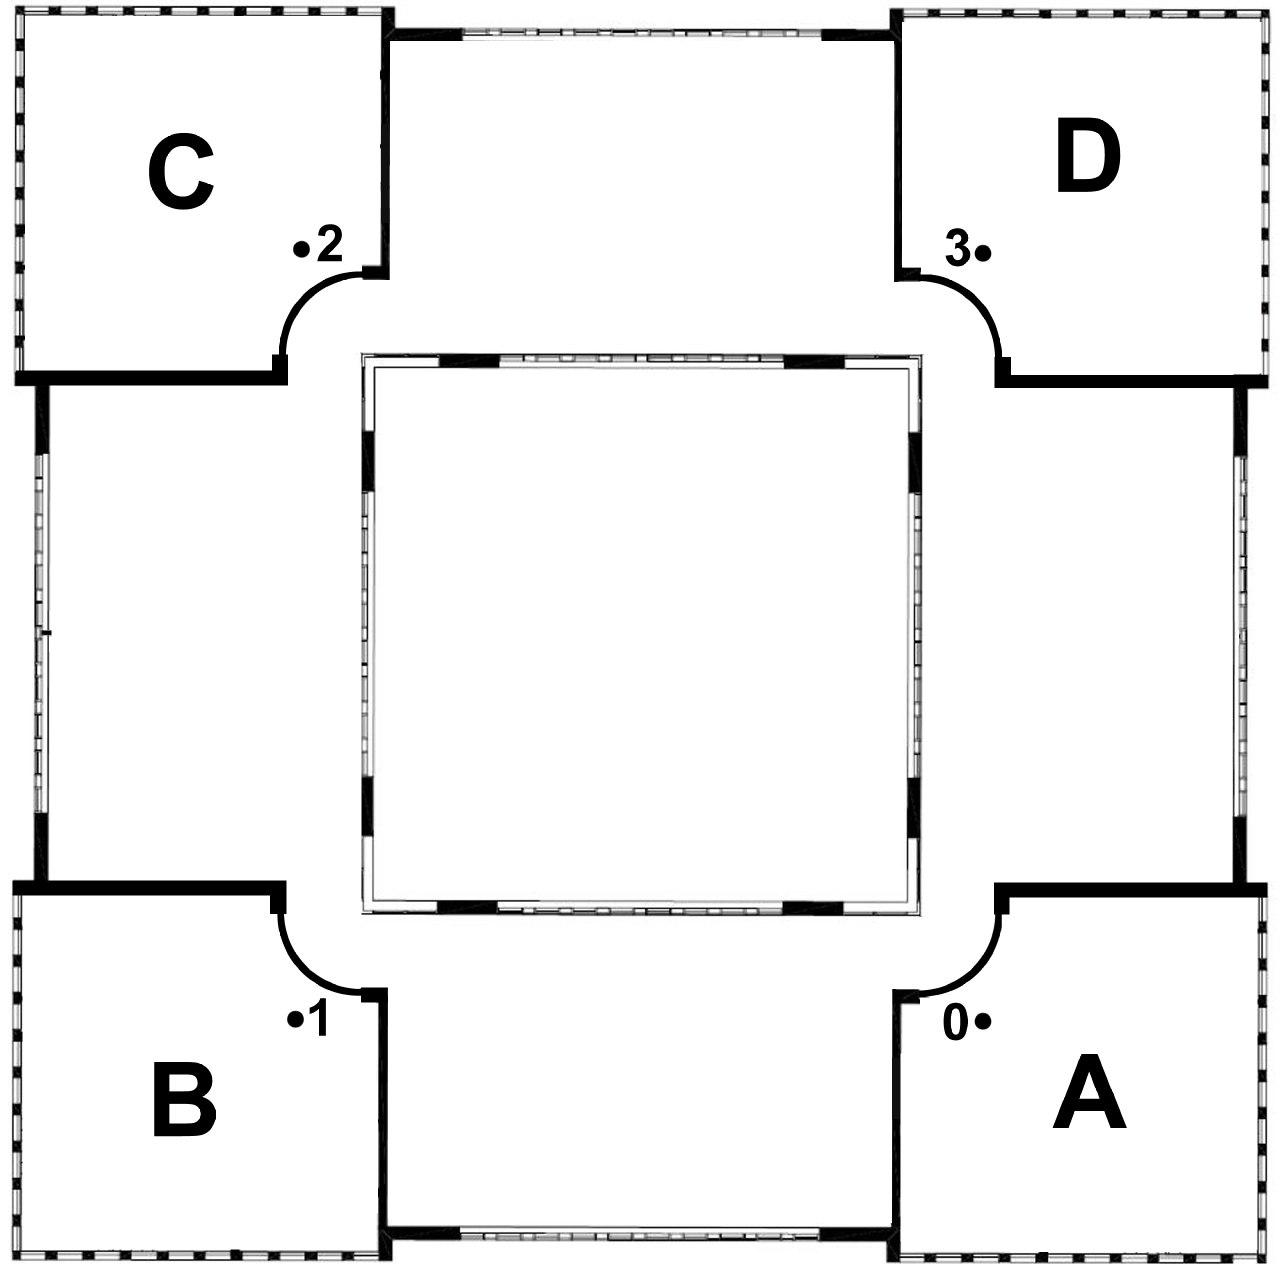
\includegraphics[width=\textwidth]{img/PianoTerra}
				\caption{Mappatura piano terra Torre Archimede}
				\label{fig:PianoTerra}
			\end{figure}						

			\begin{figure}[p]
				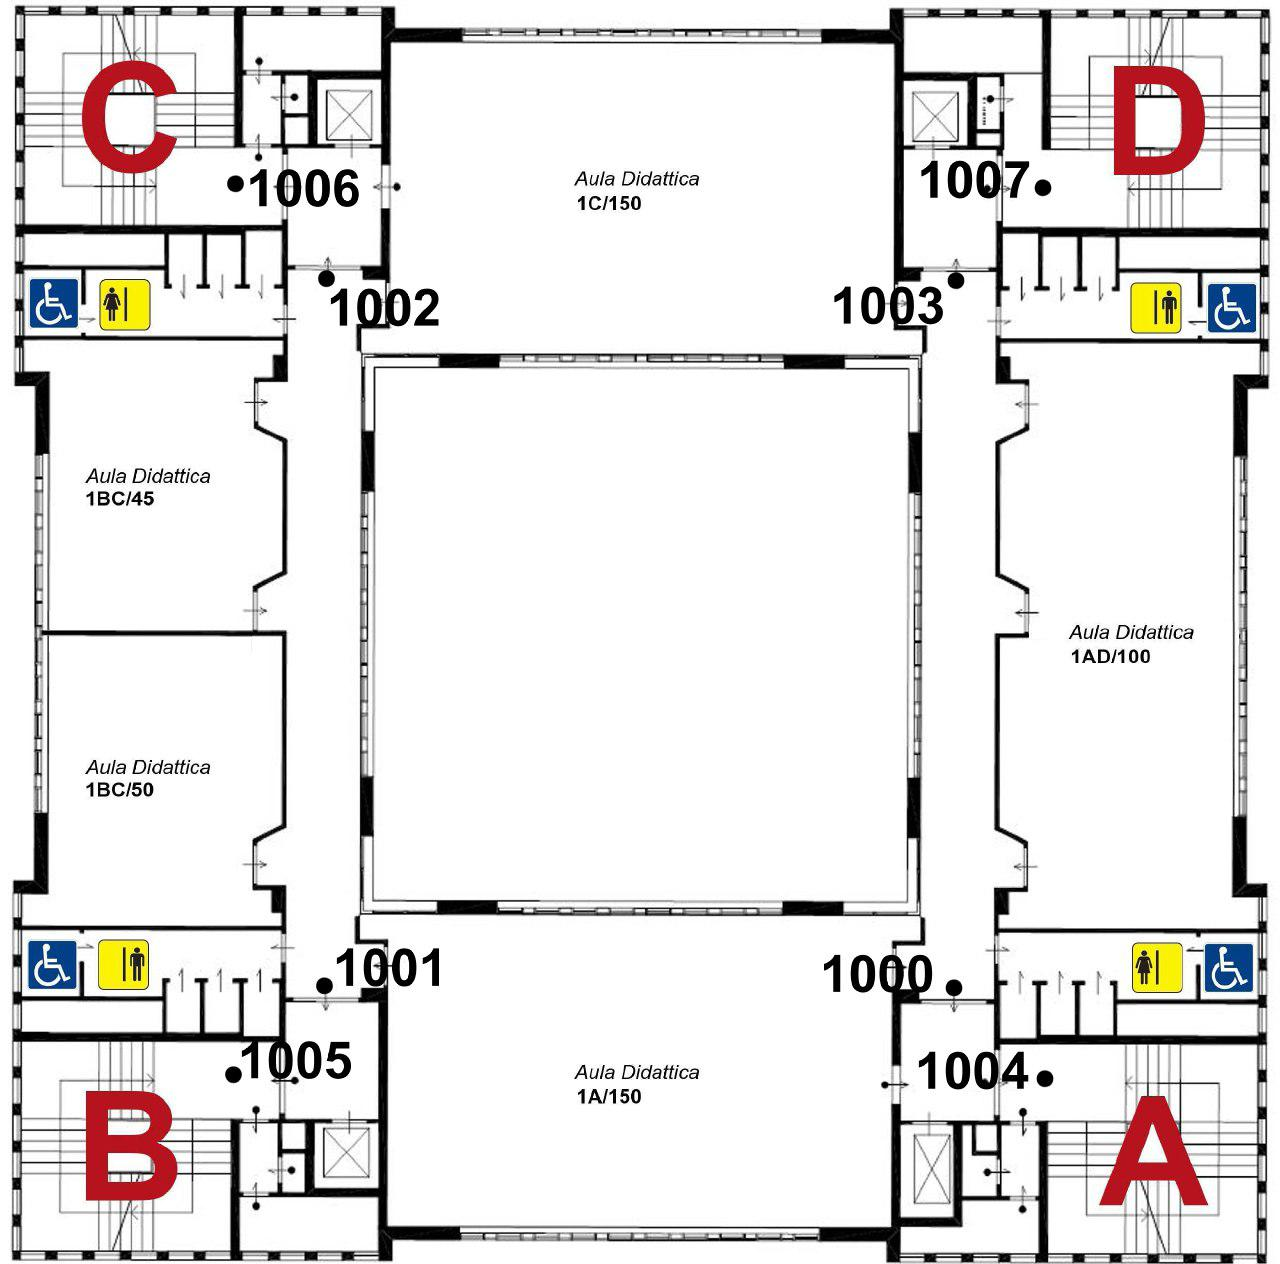
\includegraphics[width=\textwidth]{img/PrimoPiano}
				\caption{Mappatura primo piano Torre Archimede}
				\label{fig:PrimoPiano}
			\end{figure}
			
	
		\newpage
		\subsubsection{Condizioni esterne}
			Dato il numero di variabili esterne che possono influenzare l'ambiente di prova si è optato per la loro non impostazione. Ad ogni sperimentazione comunque è richiesto che nella descrizione della scelta dei questo impianto siano specificate alcune di queste variabili, in particolare una stima del numero di persone presenti.

\end{document}